\documentclass[9pt,twocolumn]{extarticle}

%% ── Packages ──────────────────────────────────────────────────────────────────
\usepackage[margin=0.75in, top=1in, bottom=1in]{geometry}
\usepackage{microtype}
\usepackage{booktabs}
\usepackage{graphicx}
\usepackage{float}
\usepackage{caption}
\usepackage{lettrine}       % drop cap
\usepackage{lineno}         % line numbers
\usepackage{titlesec}       % section formatting
\usepackage{fancyhdr}       % header/footer
\usepackage{hyperref}
\usepackage{parskip}
\usepackage{amsmath}
\usepackage{xcolor}
\usepackage{enumitem}
\usepackage{natbib}
\usepackage{authblk}

%% ── Line numbers ──────────────────────────────────────────────────────────────
\linenumbers
\renewcommand{\linenumberfont}{\tiny\sffamily}

%% ── Section formatting (numbered, bold, no extra space) ──────────────────────
\titleformat{\section}{\normalsize\bfseries}{\thesection.}{0.5em}{}
\titleformat{\subsection}[runin]{\normalsize\bfseries}{}{0em}{}[.]
\titlespacing{\section}{0pt}{8pt}{2pt}
\titlespacing{\subsection}{0pt}{4pt}{4pt}

%% ── Caption style (Fig. X. / Table X.) ───────────────────────────────────────
\captionsetup{
  labelfont  = bf,
  labelsep   = period,
  font       = small,
  justification = justified,
  singlelinecheck = false
}
\renewcommand{\figurename}{Fig.}
\renewcommand{\tablename}{Table}

%% ── Footer ────────────────────────────────────────────────────────────────────
\pagestyle{fancy}
\fancyhf{}
\renewcommand{\headrulewidth}{0pt}
\fancyfoot[L]{\footnotesize www.pnas.org/cgi/doi/10.1073/pnas.XXXXXXXXXX}
\fancyfoot[C]{\footnotesize PNAS \textbar\ \textbf{June 2026} \textbar\ vol. XXX \textbar\ no. XX \textbar\ \thepage}

%% ── No paragraph indent, small skip ──────────────────────────────────────────
\setlength{\parindent}{1em}
\setlength{\parskip}{2pt}

%% ─────────────────────────────────────────────────────────────────────────────
\begin{document}

%% ── Title block (full width) ─────────────────────────────────────────────────
\twocolumn[{%
  \begin{@twocolumnfalse}

    \begin{flushleft}
      {\LARGE\bfseries Forever Chemicals, Unequal Burdens: PFAS Contamination,\\
      Race, Income, and Property Values in New Jersey\par}
      \vspace{6pt}
      {\normalsize\bfseries Charlotte West\par}
      \vspace{2pt}
      {\small This manuscript was compiled on \today\par}
      \vspace{10pt}

      %% Abstract as bold numbered lines
      {\small\bfseries
      \begin{enumerate}[leftmargin=1.5em, label=\arabic*, itemsep=0pt, parsep=0pt]
        \item Does PFAS contamination in New Jersey drinking water disproportionately
          affect communities of color?
        \item We analyze EPA UCMR5 measurements linked to Census demographics, Zillow
          home values, and EPA ECHO facility locations at two geographic scales: ZIP codes
          and water system service areas.
        \item We find a significant positive association between PFAS exposure and
          Hispanic community share at the ZIP level ($r = 0.245$, $p < 0.001$), and
          dramatically higher shares of people of color served by water systems co-located
          with PFAS-handling industrial facilities (25.4\% vs.\ 12.3\%, $p < 0.001$).
        \item Income does not cleanly predict PFAS exposure in New Jersey; the relationship
          is nonlinear and context-dependent.
        \item Communities served by water systems with PFAS facilities inside their service
          areas have significantly lower property values (\$570k vs.\ \$816k, $p < 0.001$),
          consistent with a pollution capitalization effect.
      \end{enumerate}
      }
      \vspace{6pt}
      {\small PFAS \textbar\ Environmental Justice \textbar\ Drinking Water \textbar\ New Jersey \textbar\ Property Values\par}
    \end{flushleft}

    \vspace{12pt}
    \hrule
    \vspace{10pt}

  \end{@twocolumnfalse}
}]

%% ─────────────────────────────────────────────────────────────────────────────
\section{Introduction}

\lettrine[lines=2]{P}{er-} and polyfluoroalkyl substances (PFAS) are a class of synthetic chemicals used in industrial and consumer products since the 1940s---from firefighting foam and non-stick cookware to water-resistant textiles. Because they resist environmental degradation, PFAS accumulate in soil, water, and human tissue, earning the name ``forever chemicals'' \citep{erin2021pfas}. Exposure has been linked to kidney and testicular cancer, thyroid disease, decreased birth weight, and developmental harm including elevated rates of ADHD and Down syndrome \citep{birnbaum2020pfas}.

In the United States, drinking water is the primary exposure pathway. The EPA established a Maximum Contaminant Level (MCL) of 0.004~\textmu g/L for several PFAS compounds in 2024. Despite this, evidence suggests contamination is not distributed equally. Studies using national datasets have found that Black and Hispanic/Latino populations are 1.5 to 2 times more likely to be exposed to unsafe PFAS levels, often because they live near industrial sites, military bases, or airports where PFAS use is concentrated \citep{swanson2022ej}.

This paper extends that national literature by focusing on New Jersey, a densely industrialized state. Using water-system-level PFAS measurements linked to census demographics, property values, and EPA facility data, I ask three questions: (1) Does PFAS contamination vary by the racial composition of the communities served? (2) Does it vary by income? (3) Is proximity to PFAS-handling facilities associated with lower property values? Using two complementary units of analysis---ZIP codes and water system service areas---offers more granular evidence than prior national analyses.

%% ─────────────────────────────────────────────────────────────────────────────
\section{Data}

\subsection{Sources}
\textbf{PFAS measurements} come from the EPA's Unregulated Contaminant Monitoring Rule, Fifth Round (UCMR5), which required public water systems serving more than 3,300 people to test for 29 PFAS compounds (January 2023--December 2025). \textbf{Demographic data} come from the U.S. Census ACS 5-Year Estimates (2020--2024), tables DP05 (race/ethnicity) and S1901 (income), at the ZIP Code Tabulation Area (ZCTA) level. \textbf{Property values} are from the Zillow Home Value Index (ZHVI), extracted for December 2024. \textbf{Industrial facility locations} come from the EPA's ECHO database, filtered to PFAS-handling facilities. \textbf{PWS service area boundaries} are from the EPA's PWS Service Areas dataset (v3.0). \textbf{ZIP code shapefiles} are from the Census Bureau's 2024 TIGER/Line ZCTA file.

\subsection{Units of Analysis}
The original UCMR5 data contains one row per water system, per contaminant, per sampling event. I aggregate to two units. The \textbf{ZIP code} (ZCTA) is the primary unit for race and income analyses. The \textbf{water system service area} is the primary unit for the proximity analysis, because ECHO facility locations can be spatially intersected with service area polygons.

\subsection{Sample}
Table~\ref{tab:sample} summarizes both analysis samples. At the ZIP level, 473 of 598 NJ ZCTAs have at least one PFAS measurement. At the water system level, 245 of 558 NJ systems have PFAS records. The gap reflects the monitoring threshold: systems serving fewer than 3,300 people were not required to test.

\begin{table}[H]
\centering
\caption{Sample characteristics by unit of analysis.}
\label{tab:sample}
\small
\begin{tabular}{lcc}
\toprule
 & \textbf{ZIP Code} & \textbf{Water System} \\
\midrule
Total NJ units          & 598       & 558 \\
With PFAS data          & 473       & 245 \\
With PFAS facility inside & ---     & 204 \\
Mean PFAS (\textmu g/L) & 0.00054   & 0.00045 \\
Range (\textmu g/L)     & 0.00--0.0041 & 0.00--0.0041 \\
Exceeds EPA MCL         & 399 ZIPs  & --- \\
Mean \% POC             & 25.5\%    & 21.6\% \\
Mean median income      & \$119,755 & \$115,796 \\
Mean ZHVI               & \$630,366 & \$641,282 \\
Missing ZHVI            & 52 ZIPs   & 315 systems \\
\bottomrule
\end{tabular}
\end{table}

\subsection{Limitations}
UCMR5 only covers systems above the 3,300-person threshold, so smaller, potentially more vulnerable systems are excluded. ZCTAs are approximations of ZIP codes and do not perfectly align with water system service areas. The ECHO database may not capture all historical PFAS sources (e.g., legacy military contamination). Zillow ZHVI is missing for 315 of 558 water systems (56\%), limiting power for the property value analysis. Finally, this is a cross-sectional observational analysis; associations cannot be interpreted causally.

%% ─────────────────────────────────────────────────────────────────────────────
\section{Methods}

\subsection{Data Cleaning and Merging}
Data preparation occurs across four notebooks. \href{https://github.com/Charcharbinks28/QSS20-CW-Final/blob/main/code/00_pull.ipynb}{\texttt{00\_pull.ipynb}} downloads raw files and filters the national UCMR5 file to NJ, saving outputs to \texttt{data/01\_pulls/}. \href{https://github.com/Charcharbinks28/QSS20-CW-Final/blob/main/code/01_clean.ipynb}{\texttt{01\_clean.ipynb}} performs the ZIP-level merge: PFAS measurements are aggregated per PWSID (mean, max, MCL exceedance flag), joined to the PWSID-to-ZIP crosswalk via exact match on PWSID, then merged left on ZIPCODE with ACS race, ACS income, and Zillow ZHVI. \href{https://github.com/Charcharbinks28/QSS20-CW-Final/blob/main/code/03_clean_proximity.ipynb}{\texttt{03\_clean\_proximity.ipynb}} builds the water-system-level dataset via a spatial join (intersection) of PWS service area polygons with ECHO facility points using GeoPandas, then merges PFAS measurements and population-weighted census demographics via exact match on PWSID.

\subsection{Variable Definitions}
\textbf{mean\_pfas / max\_pfas}: mean and maximum PFAS concentration in \textmu g/L. \textbf{exceeds\_mcl\_max}: binary, 1 if max PFAS $>$ 0.004~\textmu g/L. \textbf{pct\_poc}: \% people of color ($= 100 - \%$ non-Hispanic white). \textbf{pct\_black / pct\_hispanic}: from ACS DP05. \textbf{hh\_median\_income}: median household income (USD). \textbf{zhvi}: Zillow Home Value Index (December 2024). \textbf{has\_facility}: binary, 1 if $\geq$1 ECHO PFAS facility falls within the service area polygon. \textbf{total\_facilities}: count of ECHO facilities inside the service area.

\subsection{Statistical Approach}
This is an observational, correlational study. I use three statistical tools: \textbf{Pearson correlation} ($r$) to measure linear associations between continuous variables; \textbf{independent-samples $t$-tests} to compare group means; and \textbf{OLS multiple regression} at the ZIP level to test whether the race--PFAS association persists after controlling for income. Because there is no instrument or quasi-experimental variation, I do not claim causal identification---associations may reflect shared confounders such as historical industrial land use or zoning.

%% ─────────────────────────────────────────────────────────────────────────────
\section{Results}

\subsection{PFAS Contamination and Race}
Figure~\ref{fig:race_map} shows mean PFAS concentration and \% people of color side by side across New Jersey ZCTAs. Elevated PFAS levels appear in some areas with higher non-white populations, particularly in central and northern NJ.

\begin{figure}[H]
  \centering
  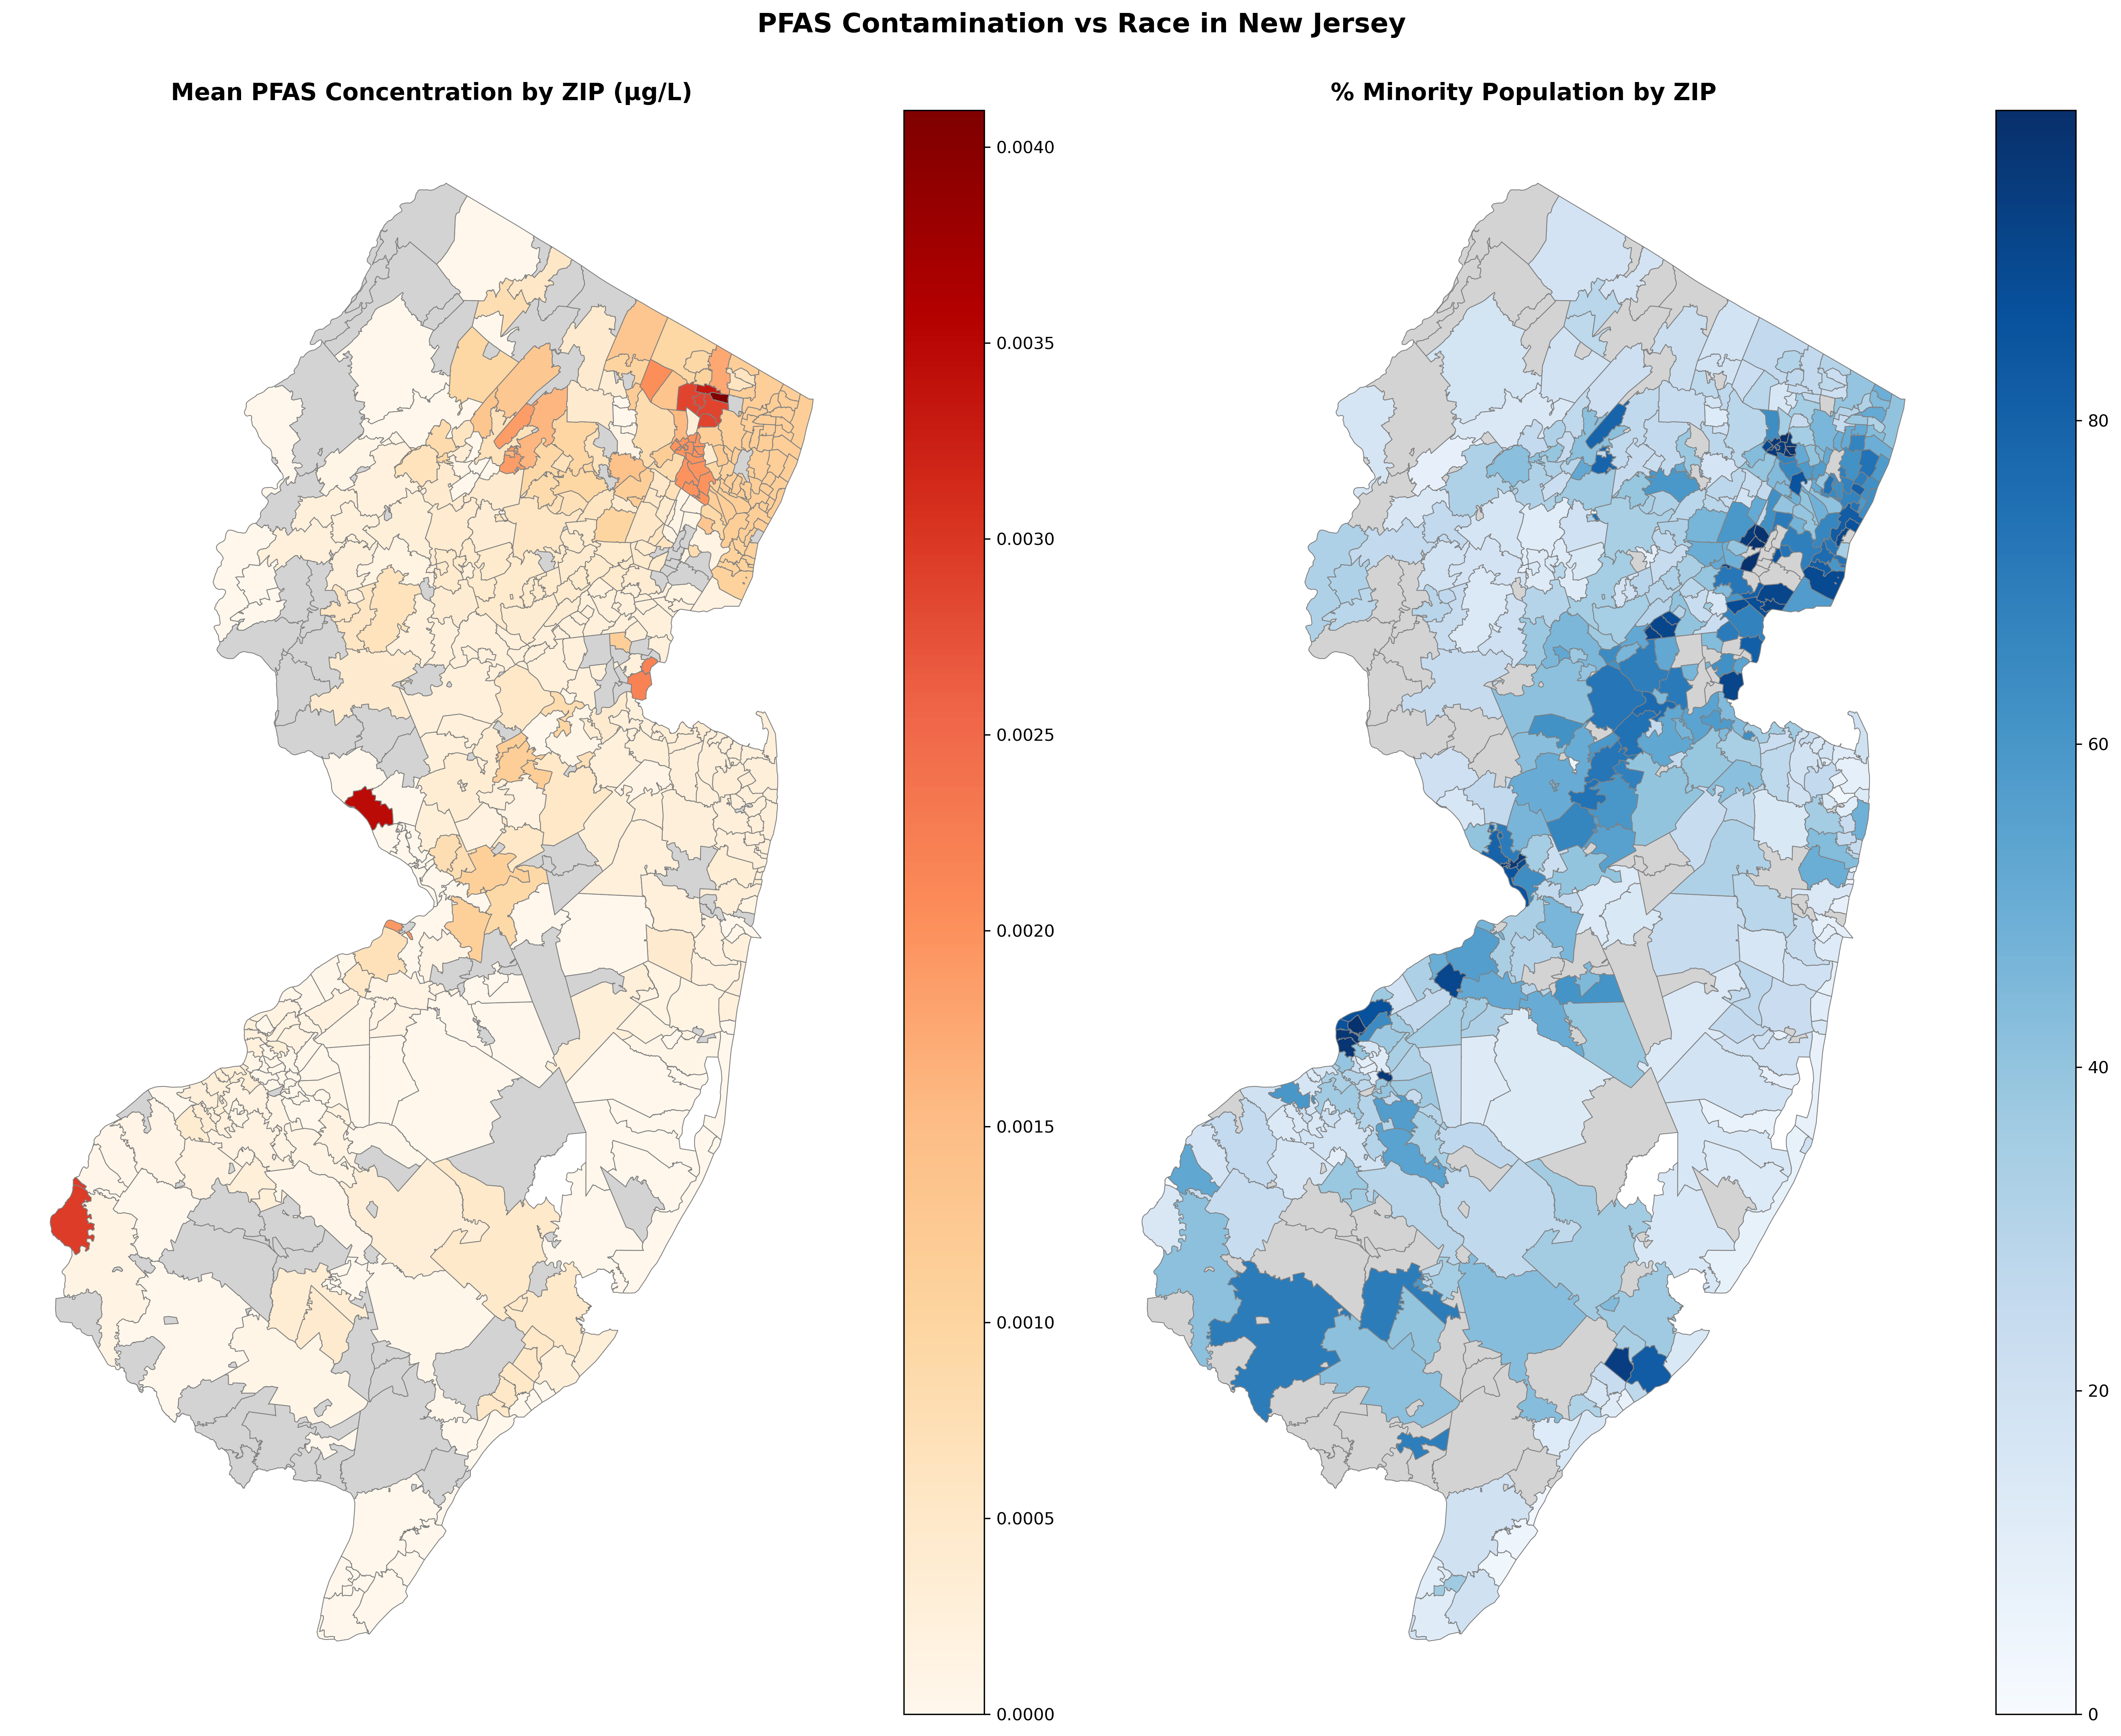
\includegraphics[width=\columnwidth]{output/nj_pfas_vs_race_map.png}
  \caption{Mean PFAS concentration (\textmu g/L) and \% people of color by ZIP code in New Jersey. Grey ZIPs lack PFAS data.}
  \label{fig:race_map}
\end{figure}

At the ZIP level, the Pearson correlation between mean PFAS and \% POC is $r = 0.123$ ($p = 0.007$)---statistically significant but modest. The effect is driven primarily by the Hispanic population: \% Hispanic correlates at $r = 0.245$ ($p < 0.001$), the strongest racial/ethnic signal. The \% Black correlation is slightly negative ($r = -0.097$, $p = 0.035$), reflecting NJ's specific geography: Black population centers like Newark and Camden are served by large municipal systems with different contamination profiles than the smaller suburban systems driving high PFAS readings. A $t$-test comparing \% POC in MCL-exceeding versus non-exceeding ZIPs yields no significant difference (15.2\% vs.\ 25.5\%, $p = 0.643$).

The cleaner signal emerges at the water system level (Figure~\ref{fig:demographics_facility}). Systems with a PFAS facility inside their service area serve far more diverse populations: 25.4\% POC vs.\ 12.3\% without ($p < 0.001$), 11.5\% Black vs.\ 5.8\% ($p < 0.001$), and 17.3\% Hispanic vs.\ 10.0\% ($p < 0.001$). These systems also have significantly higher mean PFAS (0.00052 vs.\ 0.00027~\textmu g/L, $p = 0.003$).

\begin{figure}[H]
  \centering
  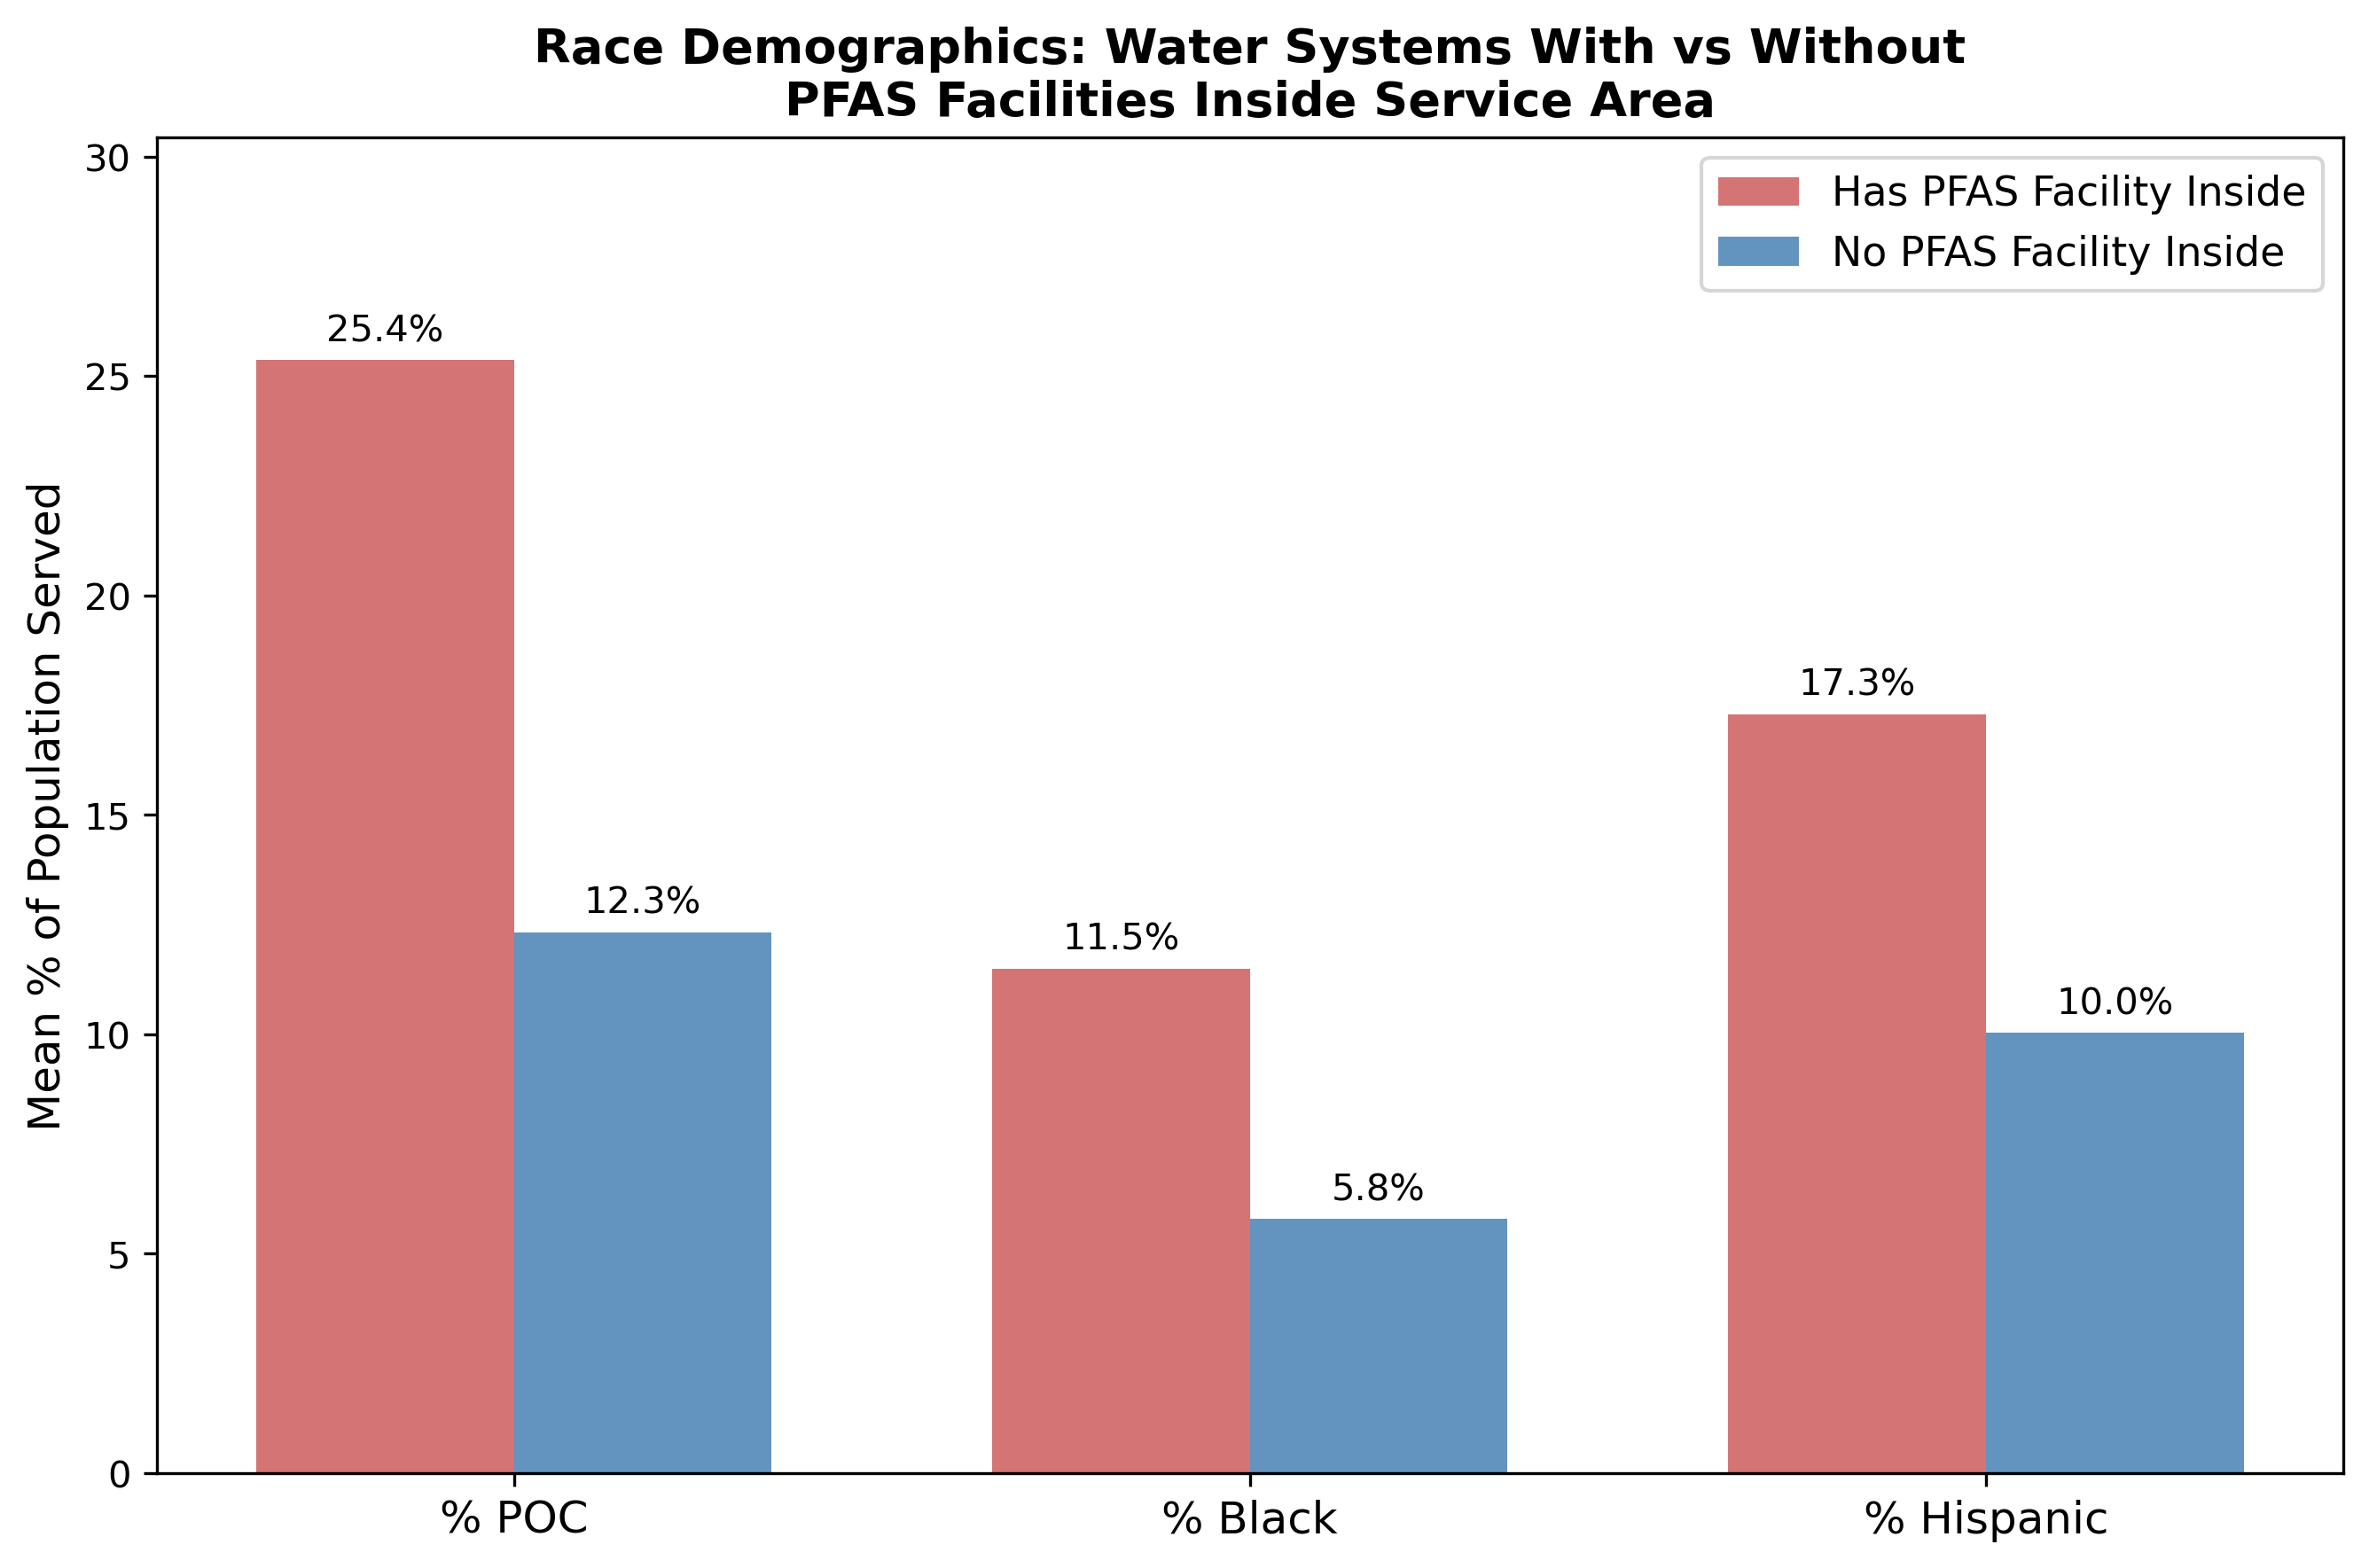
\includegraphics[width=\columnwidth]{output/demographics_facility_vs_no_facility.png}
  \caption{Mean \% POC, \% Black, and \% Hispanic for NJ water systems with vs.\ without a PFAS-handling facility inside their service area. All differences significant at $p < 0.001$.}
  \label{fig:demographics_facility}
\end{figure}

\subsection{PFAS Contamination and Income}
The relationship between PFAS and income is counterintuitive at the ZIP level: the Pearson correlation between mean PFAS and median household income is $r = 0.112$ ($p = 0.017$)---a small \textit{positive} association. This likely reflects NJ's geography, where many high-PFAS areas are affluent suburbs in Middlesex and Morris counties with long histories of industrial water use.

Decomposing income into brackets reveals more structure (Figure~\ref{fig:income_boxplot}). Households in the \$75k--\$100k and \$100k--\$150k ranges show significant \textit{negative} correlations with PFAS ($r = -0.178$, $p < 0.001$ and $r = -0.174$, $p < 0.001$), while the \$200k+ bracket shows a positive association ($r = 0.149$, $p = 0.001$). At the water system level, median household income does not differ between systems with and without a facility (\$116,598 vs.\ \$113,803, $p = 0.580$), reinforcing that income alone does not predict PFAS facility proximity in NJ.

\begin{figure}[H]
  \centering
  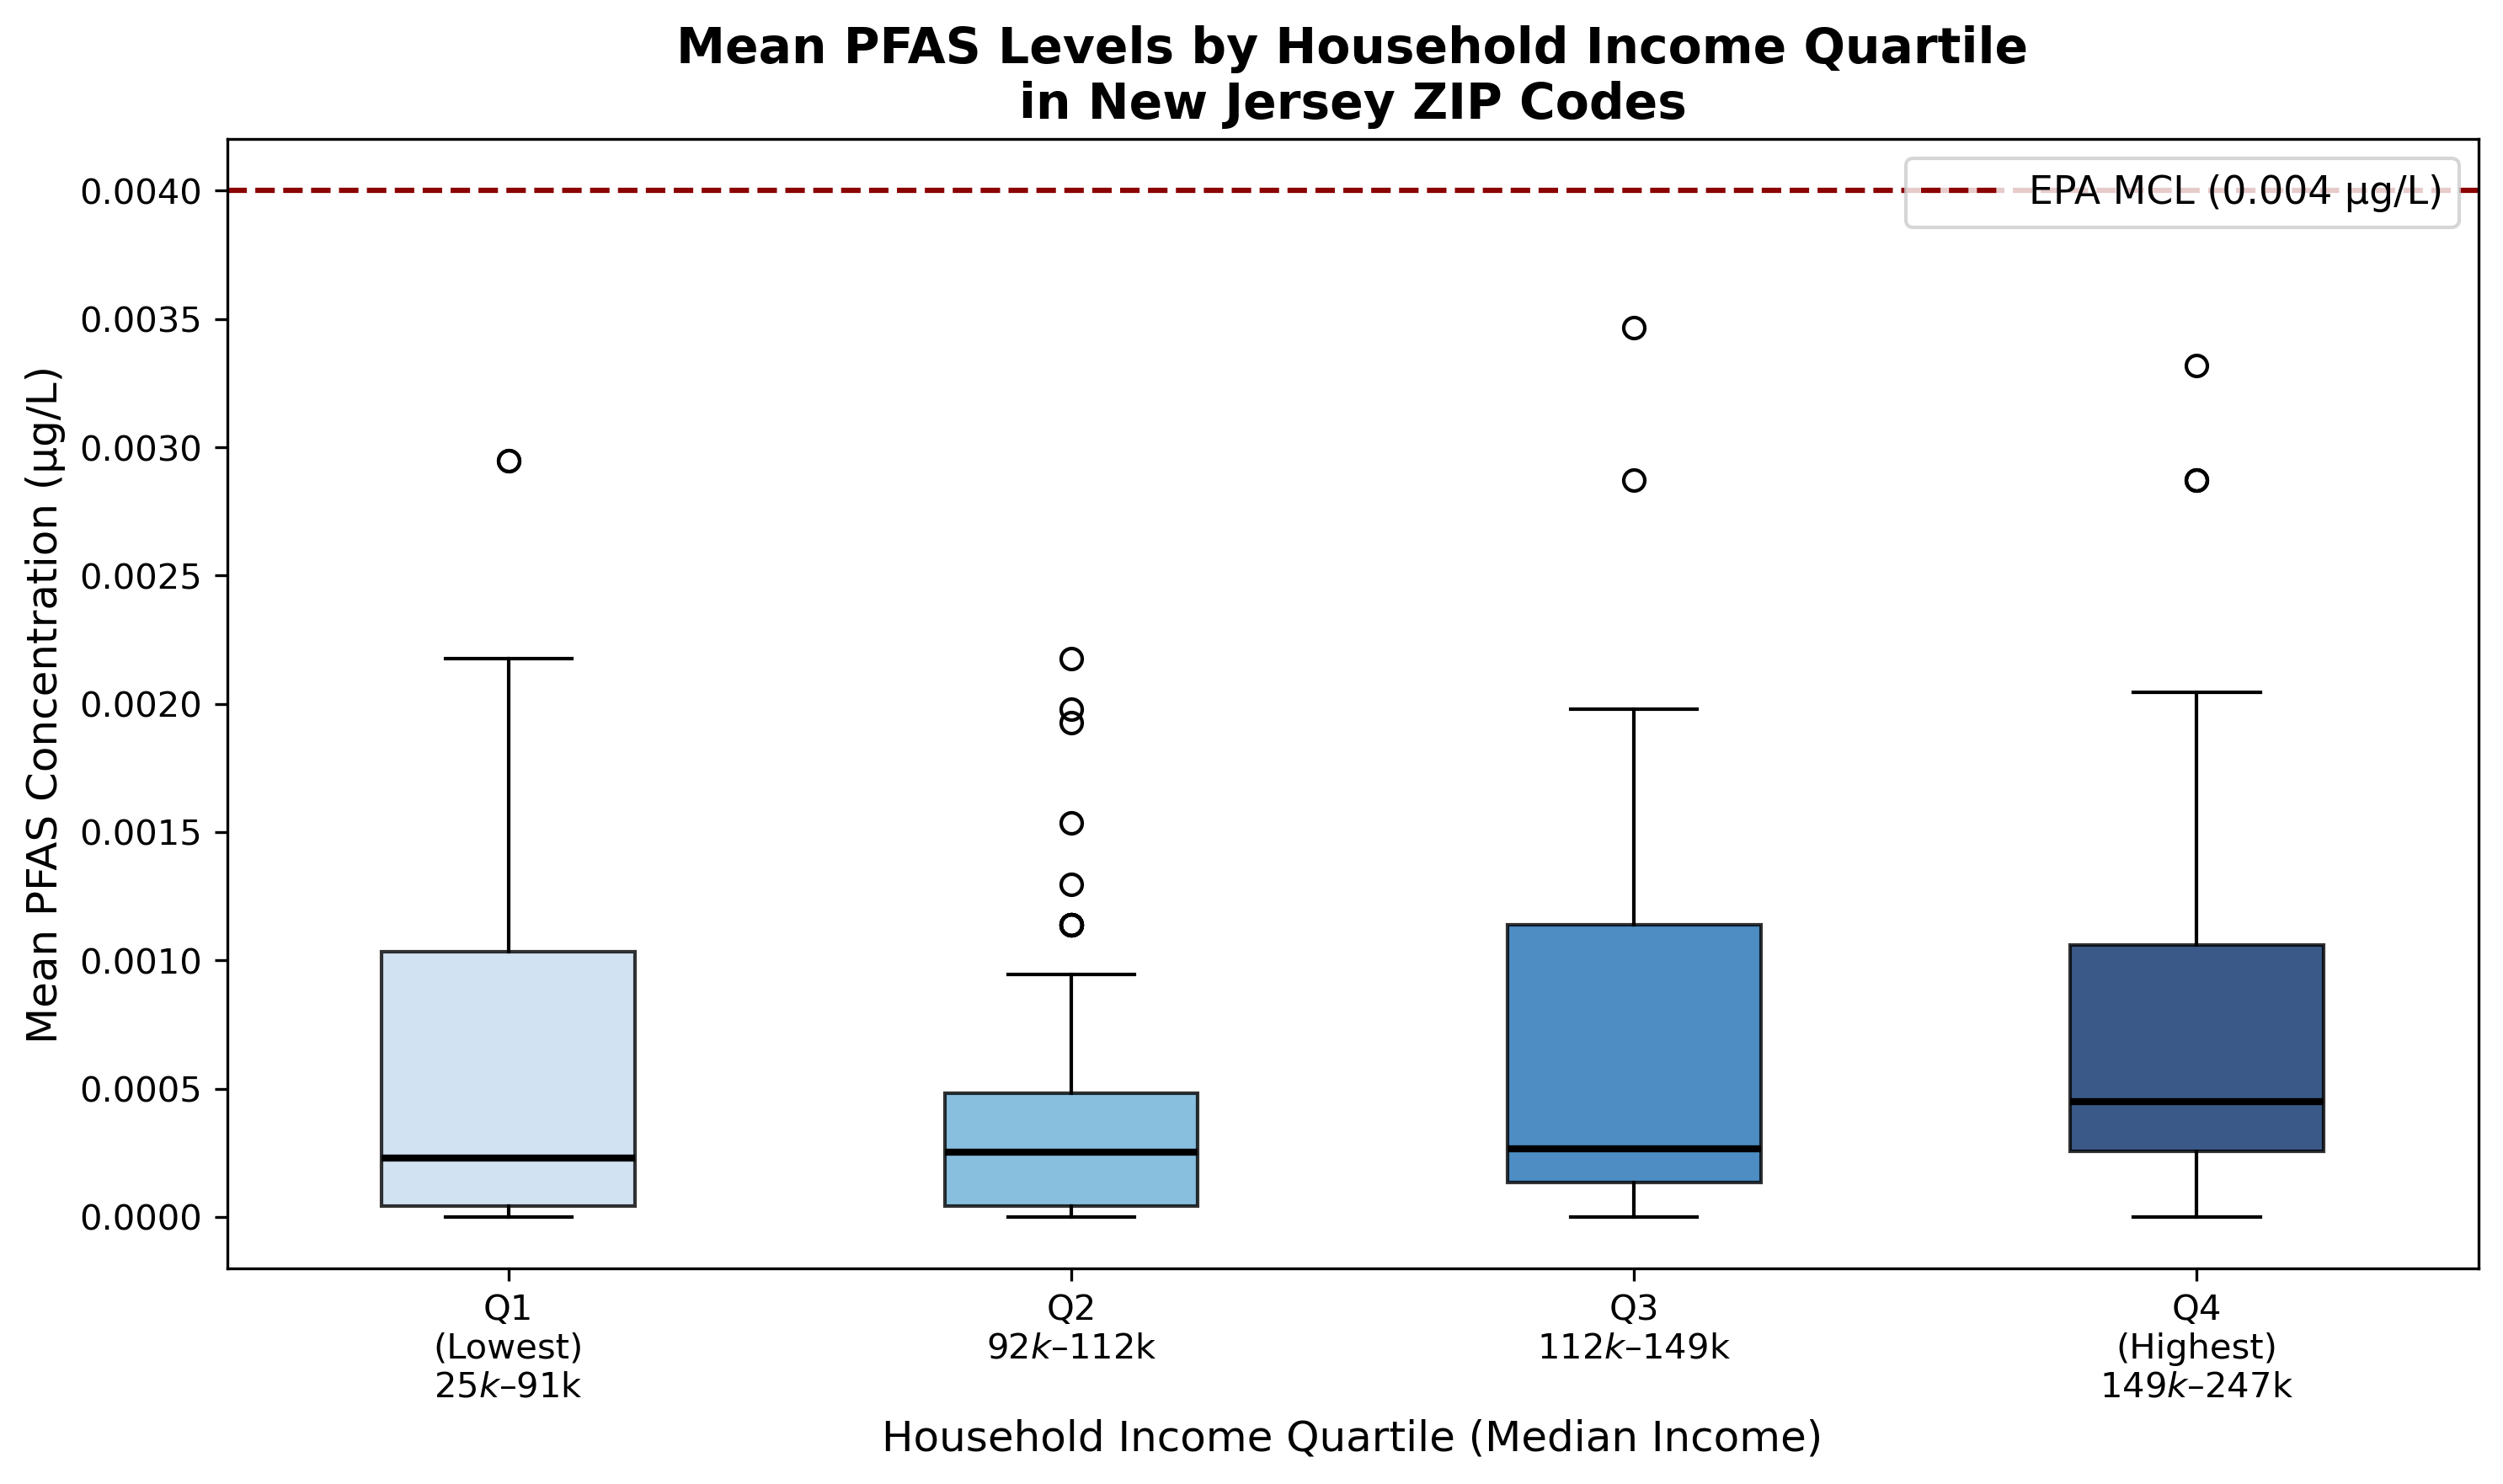
\includegraphics[width=\columnwidth]{output/pfas_by_income_quartile_boxplot.png}
  \caption{Distribution of mean PFAS by household income quartile across NJ ZIP codes. Dashed red line: EPA MCL (0.004~\textmu g/L).}
  \label{fig:income_boxplot}
\end{figure}

\subsection{Proximity to PFAS Facilities and Property Values}
The proximity analysis reveals the dataset's starkest pattern. Water systems with at least one PFAS facility inside their service area are associated with significantly lower home values: mean ZHVI of \$570,520 vs.\ \$816,164 for systems without a facility---a gap of over \$245,000 ($p < 0.001$, Figure~\ref{fig:zhvi_facility}).

\begin{figure}[H]
  \centering
  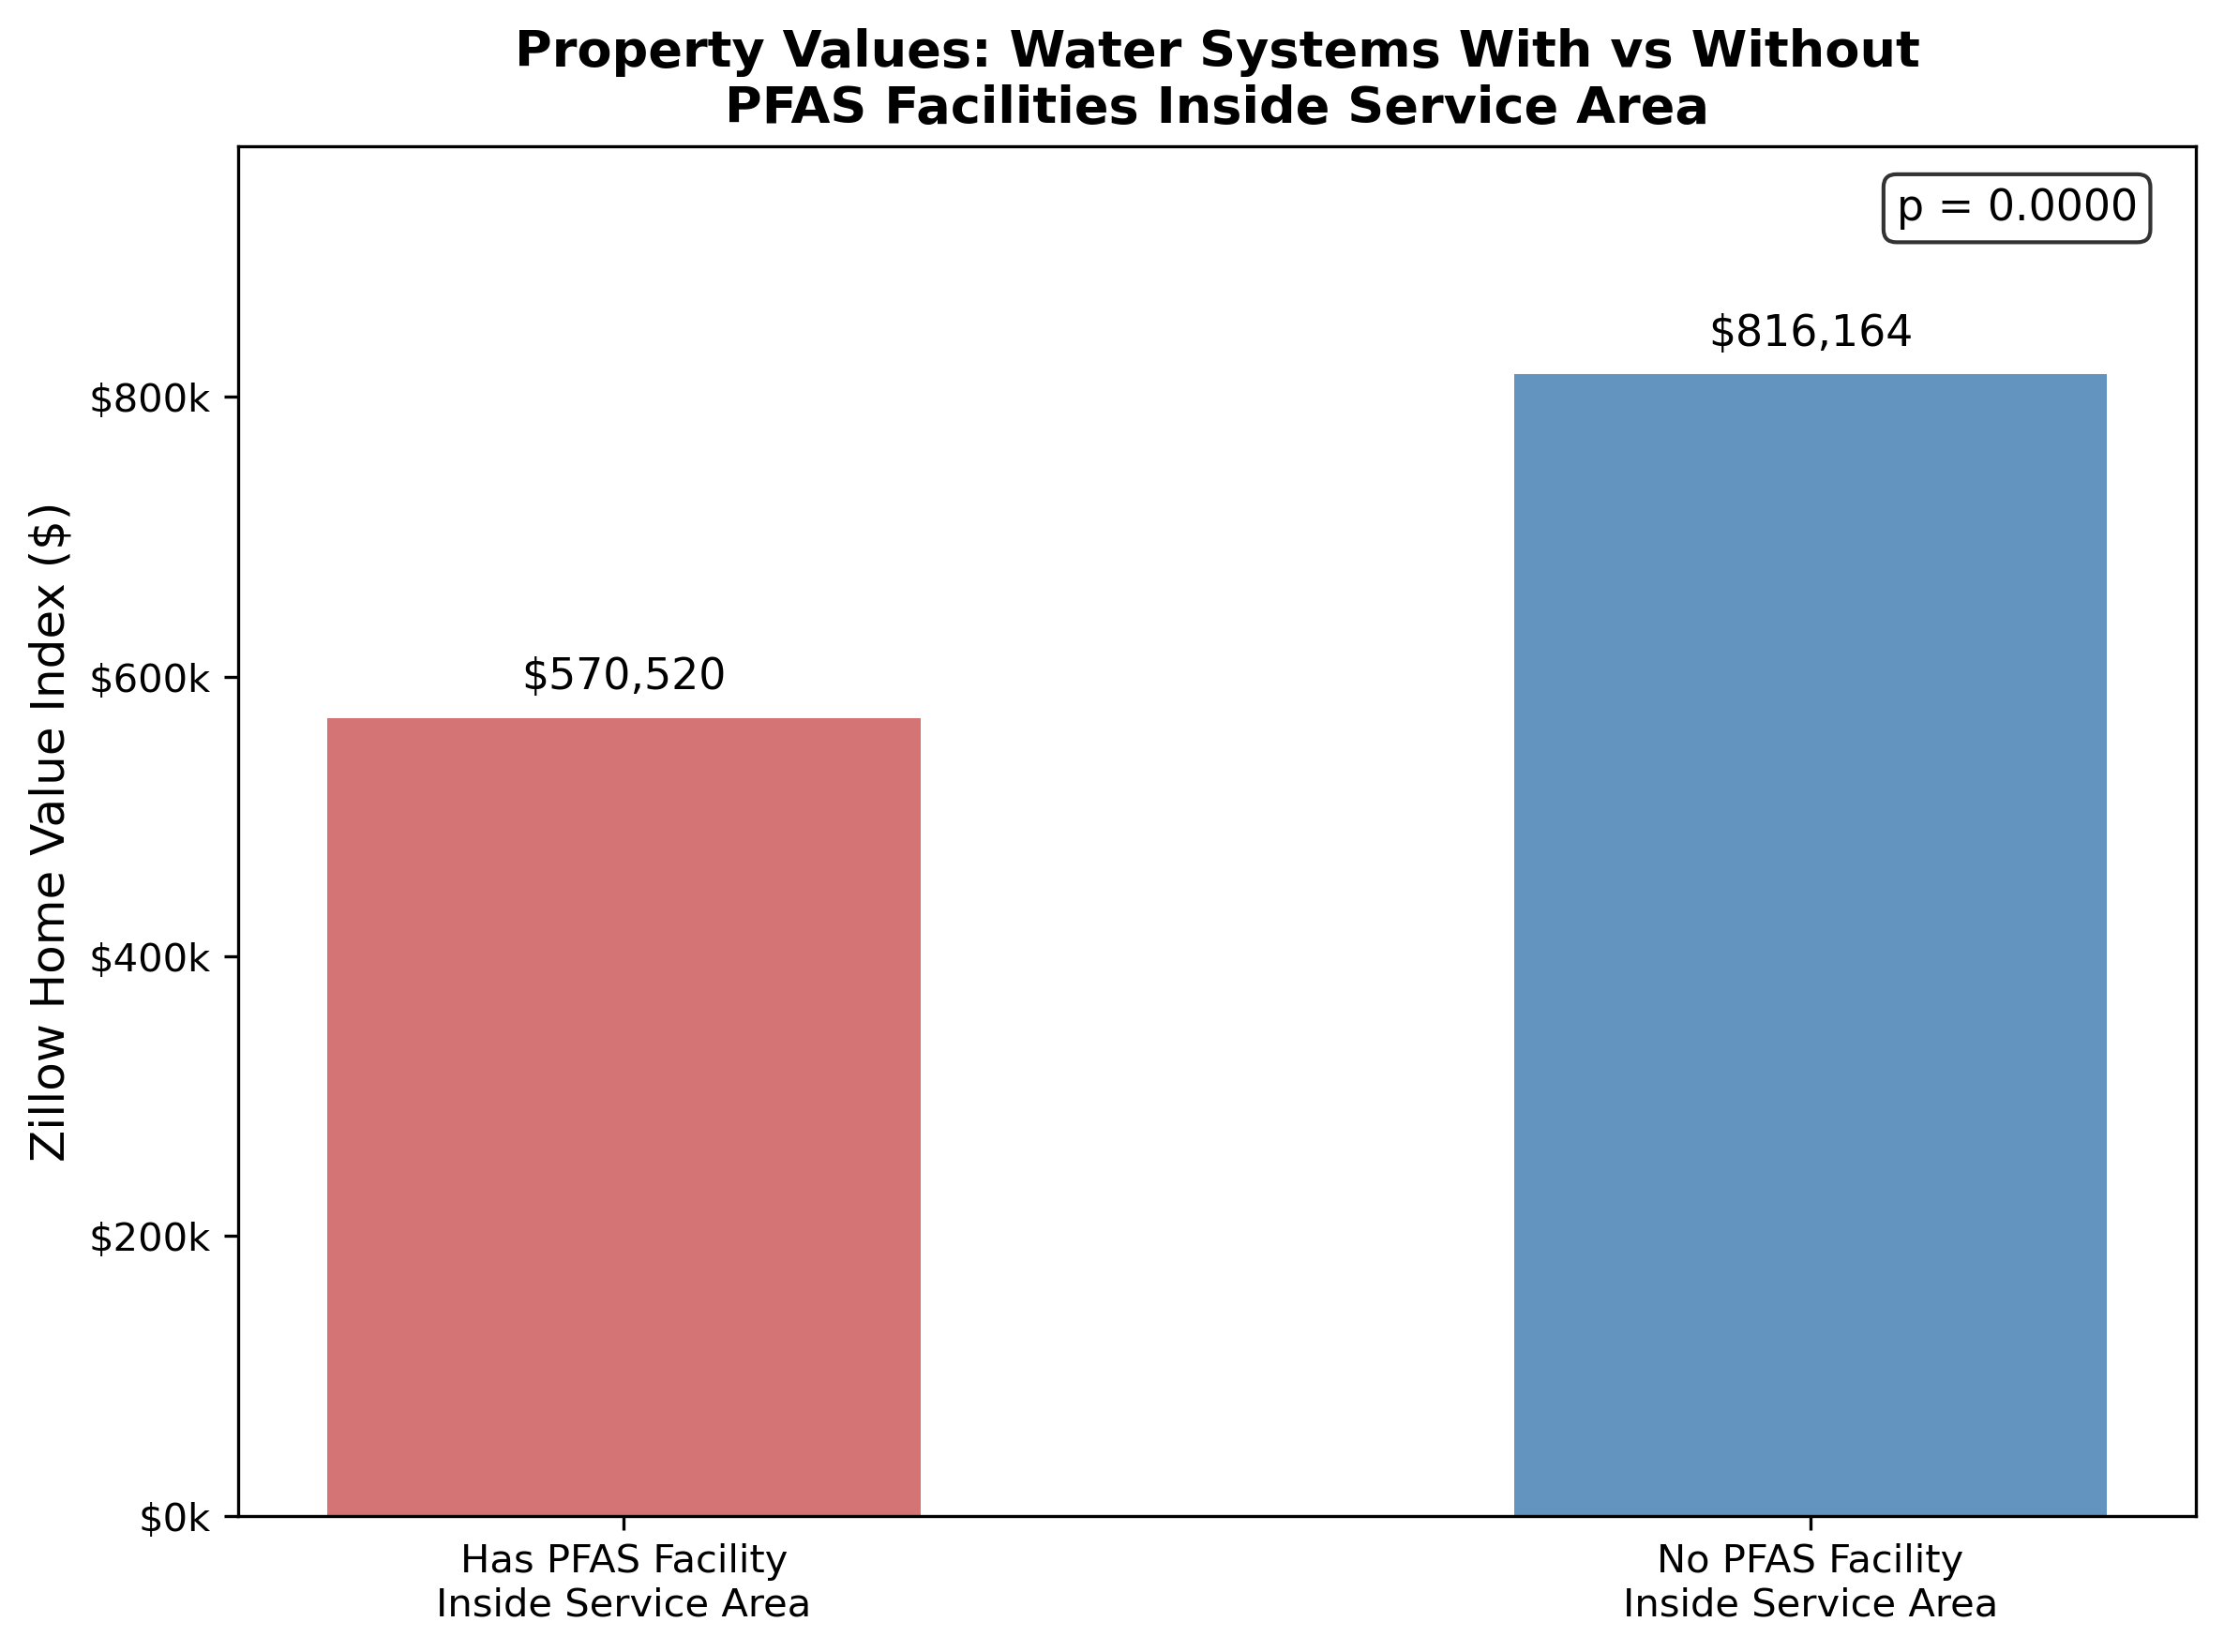
\includegraphics[width=\columnwidth]{output/zhvi_facility_vs_no_facility.png}
  \caption{Mean Zillow Home Value Index (ZHVI) for NJ water systems with vs.\ without a PFAS-handling facility inside their service area ($p < 0.001$).}
  \label{fig:zhvi_facility}
\end{figure}

At the ZIP level, the direct correlation between mean PFAS and home values is slightly positive ($r = 0.120$, $p = 0.010$), again reflecting NJ's affluent high-PFAS suburbs. However, the ZIP-level measure conflates the \textit{presence} of PFAS with its \textit{source}. When the unit shifts to the water system---where proximity to actual industrial emitters can be directly measured---the relationship reverses, consistent with a pollution capitalization effect. Figure~\ref{fig:pws_map} shows the geographic distribution of PFAS levels across service areas with facility locations overlaid.

\begin{figure}[H]
  \centering
  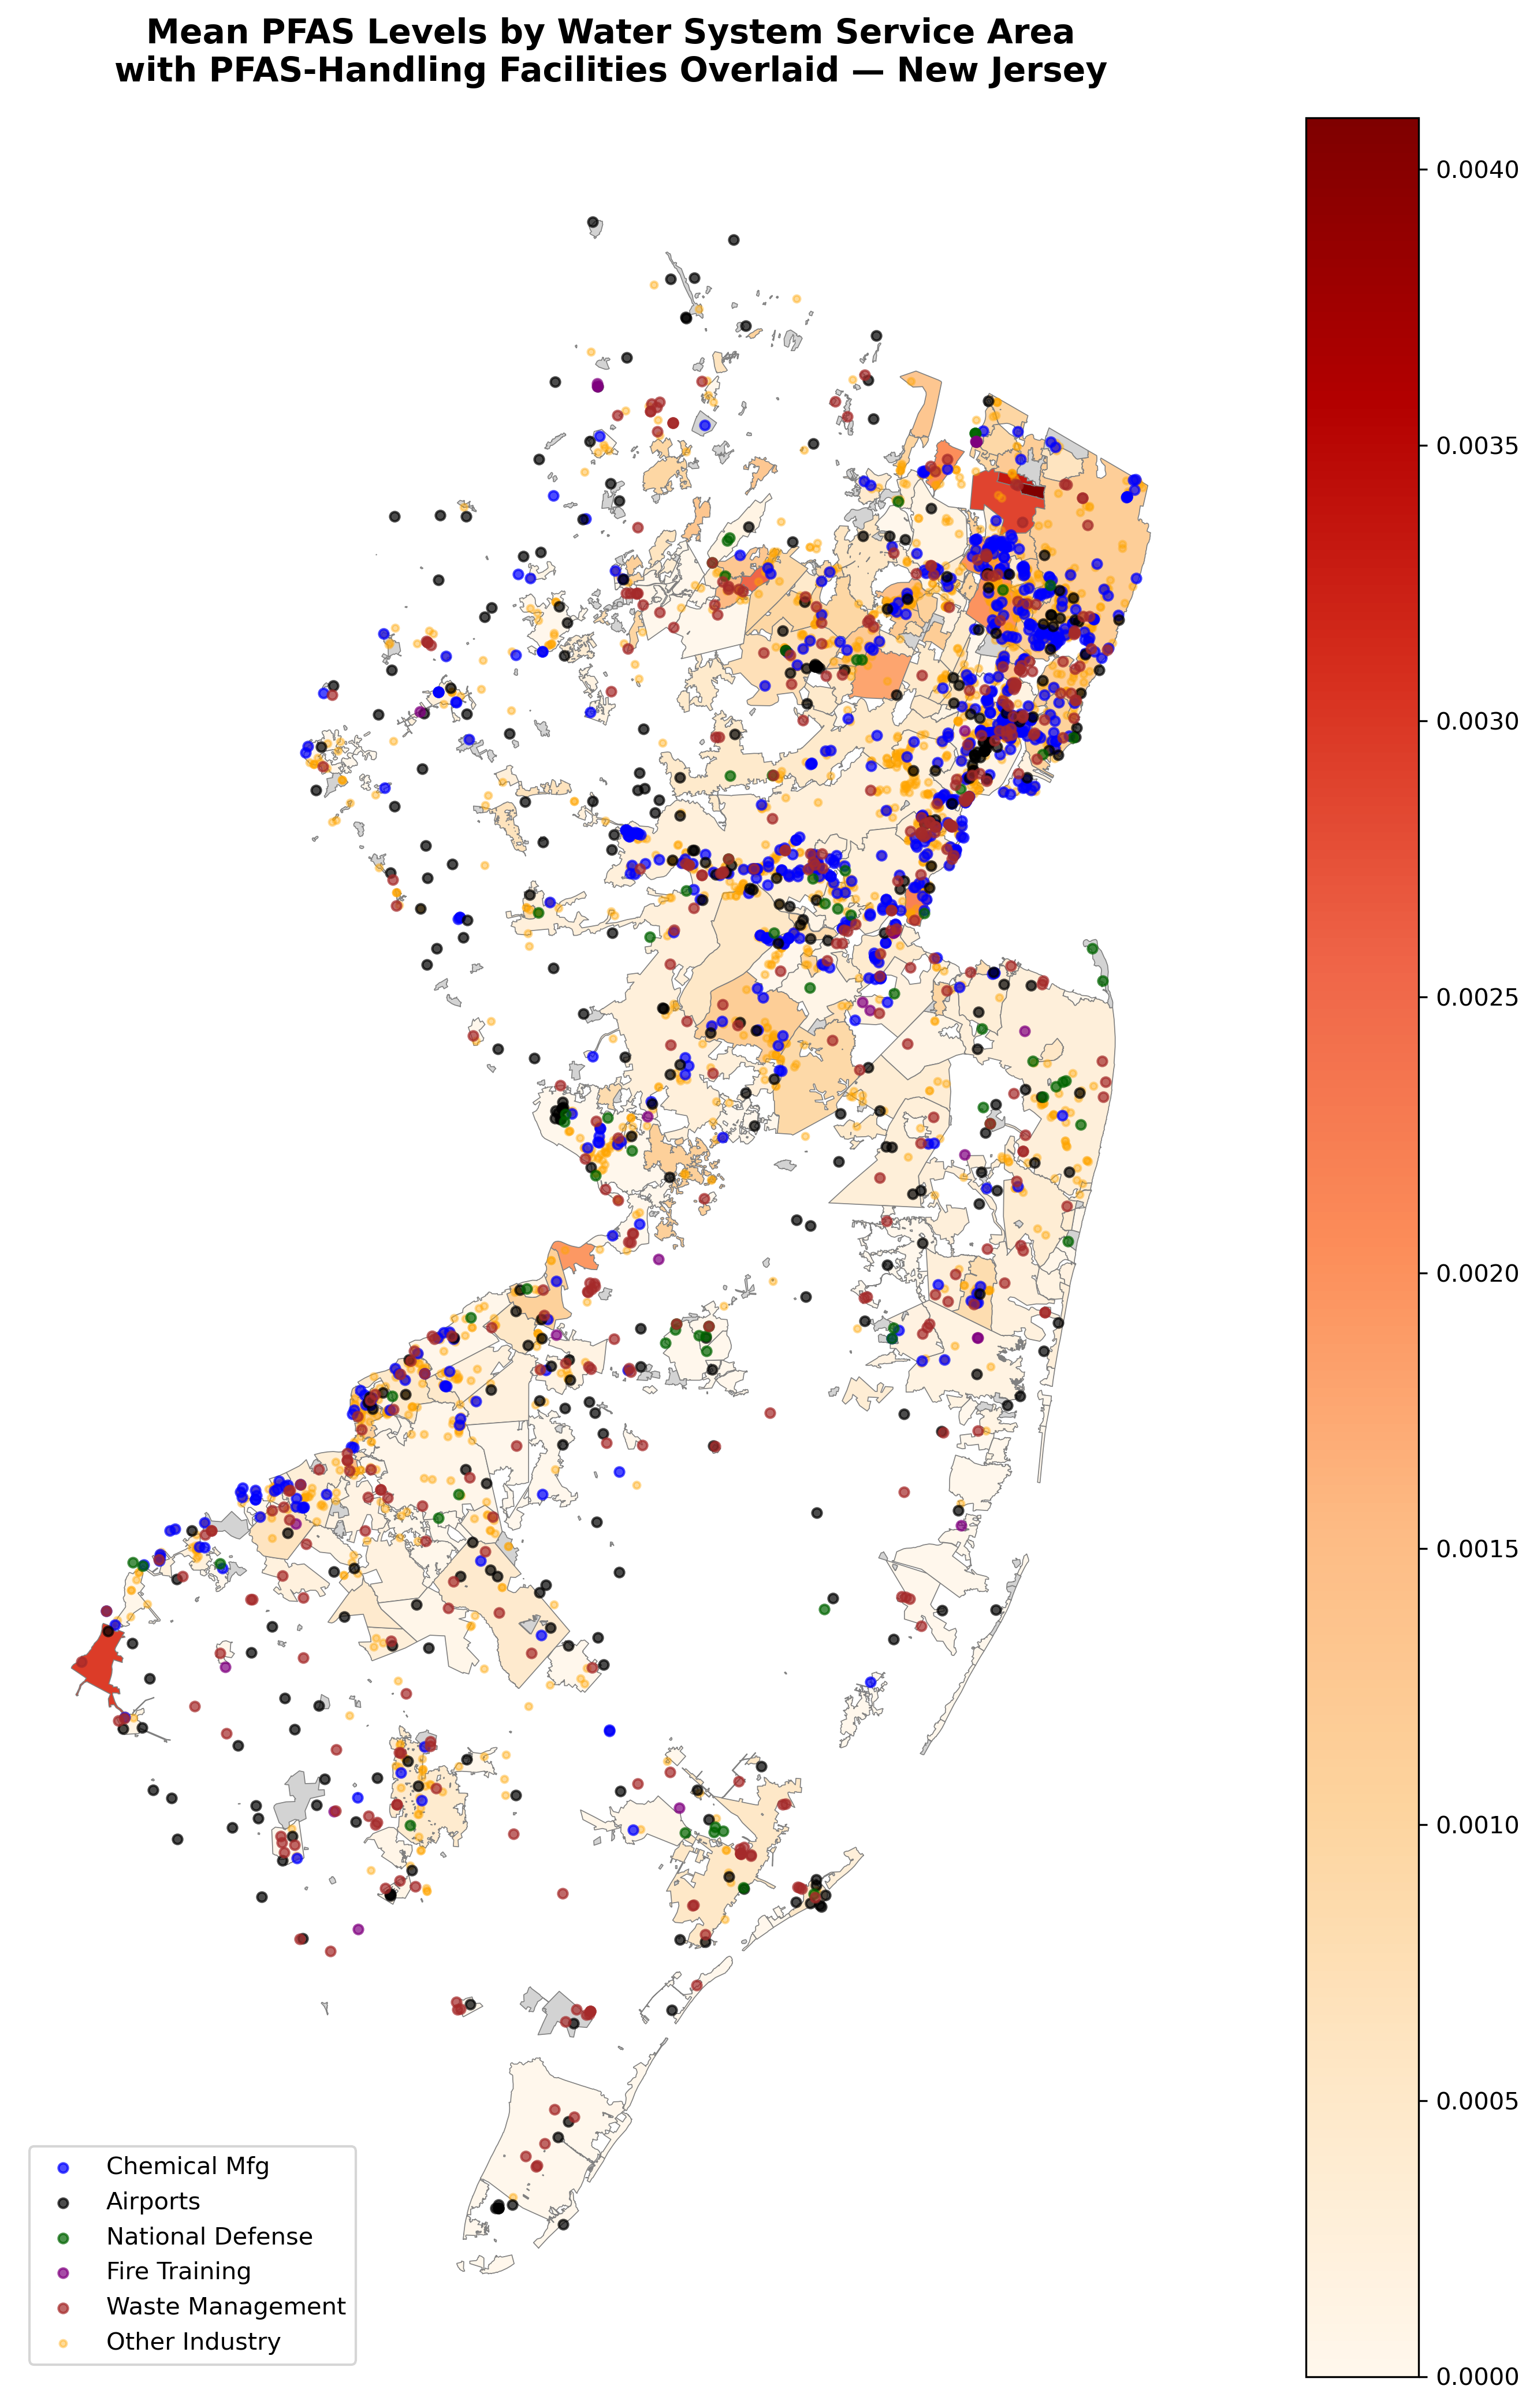
\includegraphics[width=\columnwidth]{output/pws_pfas_with_facilities.png}
  \caption{Mean PFAS by water system service area in NJ with ECHO PFAS-handling facilities overlaid by industry type. Grey areas lack PFAS data.}
  \label{fig:pws_map}
\end{figure}

%% ─────────────────────────────────────────────────────────────────────────────
\section{Discussion}

This analysis finds evidence that PFAS contamination in NJ drinking water intersects with race, though the signal is more nuanced than prior national studies suggest. Hispanic communities face disproportionately elevated PFAS at the ZIP level, while the sharpest demographic disparities appear at the facility level: water systems co-located with industrial PFAS sources serve communities with roughly twice the share of people of color. Income does not cleanly predict exposure in NJ, partly because the state's affluent suburbs overlap with high-PFAS industrial corridors. Property values, however, show a clear penalty for facility proximity---approximately \$245,000 lower on average.

Several limitations constrain interpretation. The analysis is cross-sectional and observational; no causal claim can be made without accounting for historical industrial siting, residential sorting, and local zoning. UCMR5 excludes smaller water systems, likely undercounting exposure in the most vulnerable communities. ZHVI missingness at the water system level (56\%) reduces statistical power for the property value analysis. Future work could link longitudinal PFAS data across UCMR rounds (2013--2015 vs.\ 2023--2025) to assess whether disparities have widened, and could use hedonic regression to isolate the PFAS-specific contribution to property value differences from other neighborhood characteristics.

%% ─────────────────────────────────────────────────────────────────────────────
\section{Conclusion}

This study finds evidence of racial and property-value disparities associated with PFAS contamination in New Jersey. At the ZIP level, Hispanic community share shows the strongest positive correlation with PFAS exposure. At the water system level, communities served by systems co-located with PFAS-handling industrial facilities are consistently more racially diverse and have significantly lower property values. Income shows a complex, nonlinear relationship with PFAS---one that reflects NJ's specific industrial geography rather than a simple disadvantage pattern. Together, these findings support environmental justice concerns about PFAS contamination while highlighting the importance of unit of analysis in interpreting exposure disparities.

\vspace{6pt}
\noindent\textbf{ACKNOWLEDGMENTS.} The author thanks Professor Rebecca Johnson and the QSS~20 TAs for their guidance and feedback throughout this project.

%% ── References ───────────────────────────────────────────────────────────────
\section{Works Cited}
\bibliographystyle{plainnat}
\bibliography{references}

\end{document}
